\section{Scelte implementative}
\label{cap:implementation-choices}

\subsection{Codice templatizzato}

Al fine di rendere il codice quanto più generico ed estendibile, molte delle classi e dei metodi scritti
usano i template C++, corrispondenti ai generics in Java.
I nomi ricorrenti dei tipi generici impiegati sono \textit{Label} e \textit{Weight}.
\textit{Label} denota il tipo del nome di un nodo del grafo. È istanziato come \textit{size\_t}, corrispondente a "unsigned long long", occupa almeno 64bit può rappresentare solo valori $\geq 0$.
\textit{Weight} denota il tipo del peso di un arco del grafo. È istanziato come \textit{long}, corrispondente a "signed long int",
occupa almeno 32bit.

\subsection{Rappresentazione del grafo}
\label{sub:graph-representation}

Le operazioni sui grafi di cui abbiamo bisogno sono:

\begin{itemize}
    \item Creazione di un grafo a partire da una lista di archi in input, con numero di vertici ($n$) e archi ($m$) noto a priori, e con nodi etichettati in $ 0 \leq n < n $;
    \item Enumerazione degli archi del grafo;
    \item Enumerazione dei vertici del grafo;
    \item Ottenere dei vertici adiacenti ad un nodo;
    \item Enumerazione dei vertici adiacenti ad un nodo;
    \item Aggiunta di un arco (escludendo archi duplicati di peso non minimo);
    \item Rimozione di un arco.
\end{itemize}

\noindent Le due rappresentazioni più comuni per rappresentare un grafo sono \textbf{Matrici di Adiacenza} (\textit{Adj. Matrix}) o \textbf{Liste di Adiacenza} (\textit{Adj. List}). \\
Noi abbiamo deciso invece di utilizzare una \textbf{Mappa di Adiacenza} (\textit{Adj. Map}), la quale ci permette complessità temporali migliori per le operazioni richieste a scapito di un moderato aumento della complessità spaziale, che rimane comunque \complexityNPlusM{}, lo stesso delle Matrici di Adiacenza. Nella tabella \ref{table:graph-representation-comparison} è possibile vedere un confronto tra le 3 diverse rappresentazioni di grafi possibili citate sopra. \\

L'occupazione di spazio aggiuntiva è dovuta all'utilizzo di una \textit{std::unordered\_map} e un \textit{std::unordered\_set} ausiliario. Quest'ultimo tiene traccia degli archi inseriti per permettere una rapida estrazione, modifica e cancellazione degli archi del grafo. La mappa è invece usata per mappare ogni nodo ad un'altra mappa (nodo $\rightarrow{}$ peso), usata per eliminare efficacemente i nodi duplicati di peso non minimo al momento della creazione del grafo (scelta necessaria, vista la presenza di archi duplicati nei dataset dati). L'uso di mappe ci permette inoltre di individuare ed eliminare archi in tempo \complexityConstant{} ammortizzato.

\begin{table}[ht]
\centering
    \begin{tabular}{|l|ccc|}
    \hline
    &  \multicolumn{1}{c}{Adj. Matrix} & \multicolumn{1}{c}{Adj. List} & \multicolumn{1}{c|}{Adj. Map} \\
    \hline
     Complessità spaziale   & \complexityNSquared{}  & \complexityNPlusM{} & \complexityNPlusM{} \\ \hline
     
     Creazione grafo & \complexityNSquared{}  & \complexityNPlusM{} & \complexityNPlusM{} \\
     Enumerazione archi & \complexityNSquared{} & \complexityM{} & \complexityM{} \\
     Enumerazione vertici & \complexityN{} & \complexityN{} & \complexityN{} \\
     Ottenere vertici adiacenti ad un nodo & \complexityN{} & \complexityNDegree{} & \complexityConstant{} \\
     Enumerazione vertici adiacenti ad un nodo & \complexityN{} & \complexityNDegree{} &  \complexityNDegree{} \\
     Aggiunta arco & \complexityConstant{} & \complexityConstant{} & \complexityConstant{} \\
     Rimozione arco & \complexityConstant{} & \complexityM{} & \complexityConstant{} \\
    \hline
    \end{tabular}
    \caption{Confronto di complessità spaziali (prima riga) e complessità temporali di alcune operazioni su grafi rappresentati da diverse strutture dati. "Adj. Matrix" indica "Matrice di adiacenza", "Adj. List" indica "Lista di adiacenza", e "Adj. Map" indica "Mappa di adiacenza".} \textbf{TODO: Ottenere vertici adiacenti di un nodo è O(1) in Adj Map? Sotto l'assunzione che non si restituisca un vettore o altra struttura dati forse}
    \label{table:graph-representation-comparison}
\end{table}

Il diagramma di classe in figura \ref{fig:AdjMapGraph Class} riporta gli attributi e i metodi offerti dalla classe AdjacentMapGraph.

\begin{figure}[h]
	\caption{Diagramma di classe per AdjacentMapGraph, definita in \textit{Shared/AdjacentMapGraph.h}}
	\centering
	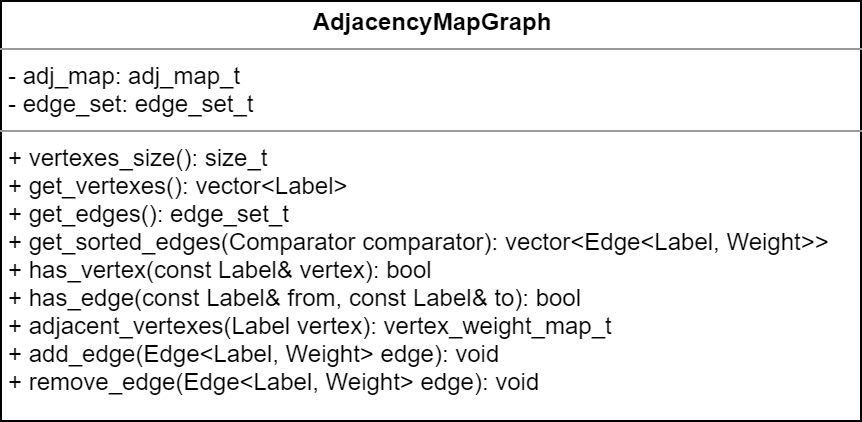
\includegraphics[width=0.7\textwidth]{./images/AdjancencyMapGrapClass.png}
	\label{fig:AdjMapGraph Class}
\end{figure}

Nella figura \ref{fig:AdjMapGraph Abstract} è riportata la trasformazione di un grafo di esempio nella relativa mappa di adiacenza che abbiamo pensato. Come è possibile notare questa mappa di adiacenza è composta da una prima mappa che elenca tutti i vertici del grafo (adj\_map\_t) e a seguire nel valore di ogni entry viene inserita una nuova mappa (vertex\_weight\_map\_t) che rappresenta gli archi del grafo: vengono elencati dunque tutti i nodi adiacenti al vertice dato con il relativo peso dell'arco. In questo modo è possibile avere tutte le operazioni di inserimento, ricerca, cancellazione e update in tempo costante, a discapito di una complessità spaziale più elevata. 

\begin{figure}[h]
	\caption{Rappresentazione della mappa di adiacenza}
	\centering
	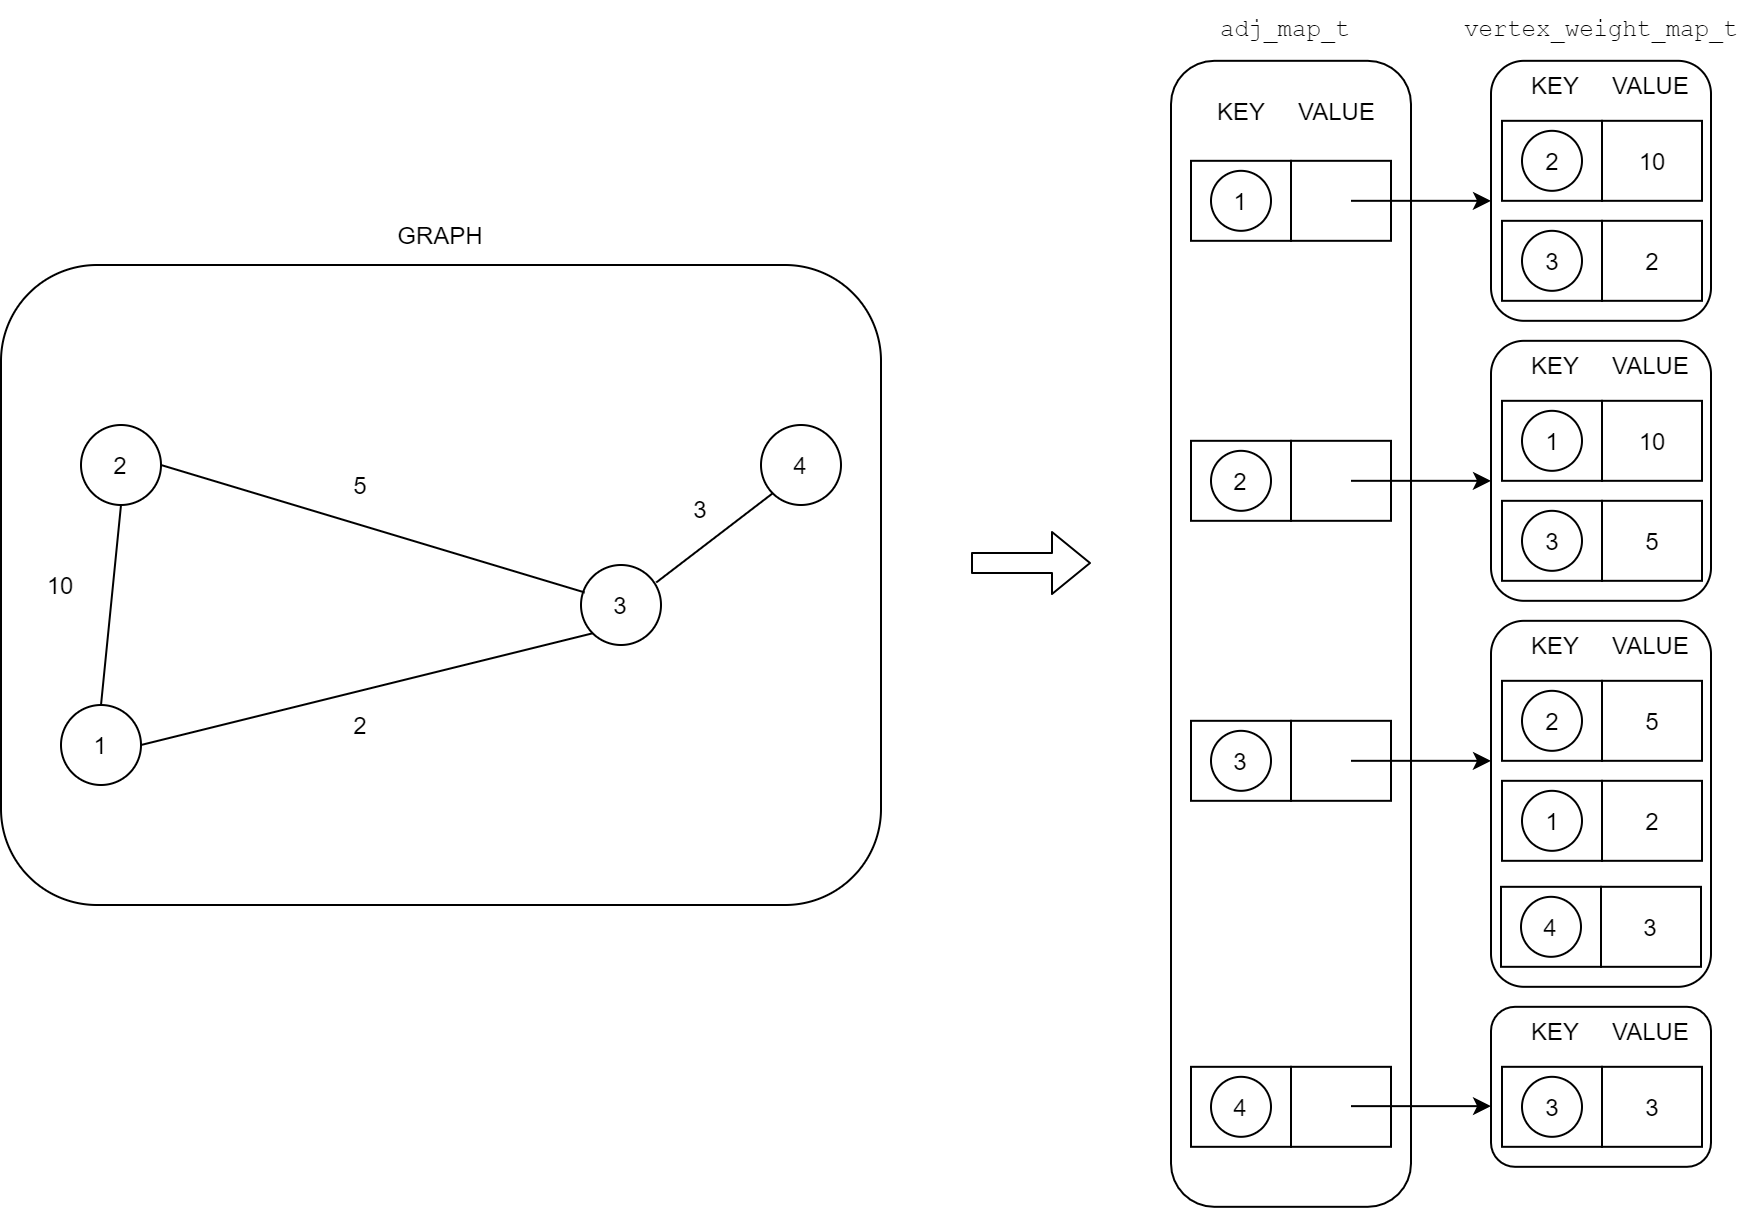
\includegraphics[width=0.7\textwidth]{./images/AdjMapGraphAbstract.png}
	\label{fig:AdjMapGraph Abstract}
\end{figure}

Nonostante la mappa di adiacenza sarebbe già stata sufficiente per salvare tutte le informazioni necessarie alla rappresentazione di un grafo, in alcune operazioni risulta essere lenta. L'esempio di operazione che ci ha spinto ad inserire una nuova struttura dati (unordered\_set in questo caso) è il metodo per ritornare tutti gli archi di un grafo in quanto tale metodo se implementato avendo a disposizione la sola mappa di adiacenza prevederebbe in maniera semplice la scansione dell'intera mappa di adiacenza, con l'inserimento degli archi via via che si incontra un nuovo vertice. Tale semplice implementazione però porterebbe alla creazione di un vettore in cui se sussiste un arco tra un vertice 2 e un vertice 3 (come nell'esempio in figura~\ref{fig:AdjMapGraph Abstract}), al vettore verrebbe aggiunto sia l'arco 2 $\rightarrow$ 3 che 3 $\rightarrow$ 2. \\

% Le cose si complicano maggiormente infatti se si restringe la richiesta di non restituire gli archi doppi come abbiamo già osservato. A tale proposito si potrebbe ricercare l'eventuale presenza di tali archi doppi ed eliminarli di conseguenza, ma il tutto richiederebbe maggiori operazioni e dunque un maggior complessità temporale.\\

% Per tali ragioni è stato deciso di affiancare alla mappa di adiacenza, un'apposita struttura dati che permettesse di tenere traccia degli archi e di avere tempi di esecuzione costanti per le operazioni di aggiunta, rimozione e ricerca. Così facendo è possibile garantire che l'operazione di restituzione degli archi singoli di un grafo abbia tempo O(m) se si richiede di restituire un vettore, o addirittura O(1) se si richiede la restituzione di un puntatore a tale struttura.

E' stato scelto dunque di utilizzare come struttura dati da affiancare unordered\_set perché oltre ad avere le caratteristiche richieste, se appositamente configurata permette di garantire l'assenza di archi doppi, compresi quelli visti nell'esempio precedente (ossia 2 $\rightarrow$ 3 e 3 $\rightarrow$ 2). Per fare ciò è stato dunque opportunamente configurato l'operatore di uguaglianza e la funzione di hash, in  modo che archi equivalenti abbiamo la stessa funzione di hash e siano riconosciuti come uguali, evitando così l'inserimento di un arco doppio visto che  unordered\_set non prevede elementi doppi al suo interno.\\

Una rappresentazione astratta di tale struttura è possibile visualizzarla nella figura~\ref{fig:edges_set}, dove è possibile notare che se viene richiesto l'inserimento di un arco 3 $\rightarrow$ 2 ove già presente un arco 2 $\rightarrow$ 3 questo non viene inserito da unordered\_set.\\

\begin{figure}[h]
	\caption{Visualizzazione astratta di edges\_set}
	\centering
	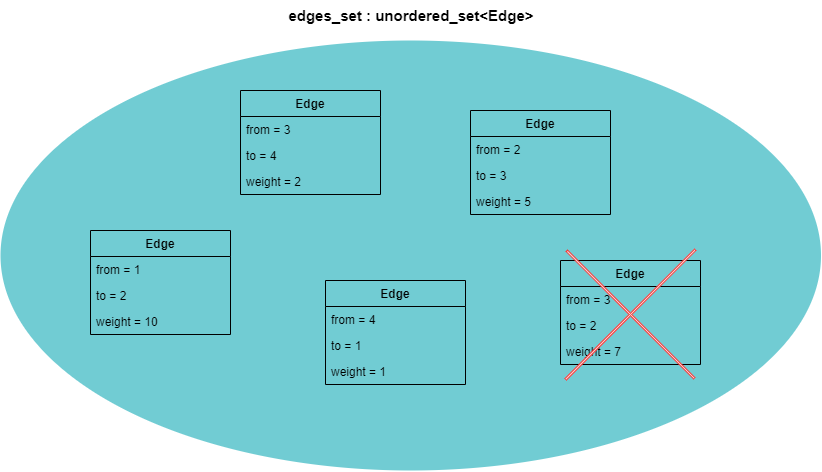
\includegraphics[width=0.7\textwidth]{./images/edges_setAbstract.png}
	\label{fig:edges_set}
\end{figure}

L'ultimo problema non ancora affrontato riguarda la possibilità di inserire un arco doppio tra due nodi uguali (come richiesto da problema), con la differenza che questi 2 archi hanno un peso diverso. Siccome la nostra implementazione non prevede la presenza di tali archi doppi, la funzione add\_eddge() si occupa di verificare l'eventuale presenza di un arco già inserito e di conseguenza i relativi pesi, per andare a modificare il peso qualora il peso del nuovo arco sia inferiore al peso dell'arco precedentemente già inserito. Per fare questo ad ogni aggiunta di un nuovo arco si va a verificare nella lista di adiacenza l'esistenza di un arco per quei due vertici:
\begin{itemize}
	\item \textbf{se l'arco era già stato aggiunto:} si confrontano i due pesi e si aggiorna il peso dell'arco solo nell'eventualità in cui il nuovo peso sia inferiore a quello già presente nella lista di adiacenza. Dopodiché se c'è stato un aggiornamento si aggiorna anche il relativo unordered\_set, eliminando l'arco precedente e si ri-aggiunge l'arco con il nuovo peso. 
	\item \textbf{se l'arco non era già stato inserito:} si inserisce l'arco sia nella lista di adiacenza che nell'unordered\_set.
\end{itemize}

\noindent Le operazioni di inserimento nei container \textit{std::unordered\_set} e \textit{std::unordered\_set} hanno complessità temporale \complexityConstant{} ammortizzata. Tuttavia, dal momento che sappiamo a priori il numero di vertici da inserire in \textit{adj\_map} e il numero di archi da inserire in \textit{edge\_set}, abbiamo preallocato un numero di bucket sufficienti ad evitare costosi \textit{rehash} in entrambi i casi.

\subsubsection {Costruzione del Grafo}

\textit{Shared/adjacency\_map\_graph\_factory.h} definisce una funzione di utilità che scorre tutte le righe del file in ingresso, salva gli archi in un vettore temporaneo, e lo trasferisce tramite \textit{move semantics} ad un nuovo oggetto di tipo \textit{AdjacencyMapGraph}. La mappa di adiacenza interpreta il grafo come spiegato nella sezione \ref{sub:graph-representation}. \\

\noindent \textbf{NOTA}: il valore dei nodi di ogni grafo è decrementato di 1 in fase di lettura del dataset di input.
Questo semplifica e rende più leggibile l'implementazione di alcune strutture dati (ad esempio i Disjoint Set) e la costruzione dell'MST con Prim.

\subsection{Strutture Dati}

Tutte le strutture dati elencate di seguito sono definite nella cartella \textit{Shared}.
Ove possibile, per la nomenclatura dei metodi abbiamo cercato di seguire lo stesso standard dei container STL di C++.
Inoltre, le strutture dati usate sono sempre preallocate in memoria quando possibile, evitando rehashing e riallocazioni dispendiose. Questo significa che la maggior parte delle operazioni indicate con \complexityConstant{} ammortizzato siano in realtà totalmente costanti nella pratica.

\subsubsection{Heap}

\textit{Heap.h} contiene la definizione astratta di una generica Heap.
Gli elementi della Heap sono salvati in un \textit{std::vector}.
Per generalizzare il concetto di MinHeap/MaxHeap, la classe usa un comparatore binario booleano. Se il funtore dato in input alla classe è
\textit{std::greater<>}, la struttura dati avrà la semantica di una Min Heap; viceversa, con il comparatore \textit{std::less<>} si avrà la semantica di una Max Heap.

\paragraph{Ottimizzazioni}\mbox{} \\

\noindent Il parametro template \textit{IsAlreadyHeap} è usato per evitare di costruire la Heap se l'utente specifica il container dato in input alla struttura dati rispetta già la proprietà di essere una Heap. Il controllo su questo flag booleano avviene a compile-time. Questa ottimizzazione garantisce un risparmio di tempo pari a \complexityN{}, ed è usata nell'implementazione dell'algoritmo di \textbf{Prim}. \\

\noindent I metodi che ripristinano la prioprietà di Heap (\textit{heapify\_up} e \textit{heapify\_down}) sono definiti in modo iterativo invece che ricorsivo, ottenendo performance migliori a parità di input. \textbf{TODO: ne siamo ancora convinti al riguardo??}

\subsubsection{Binary Heap}

\textit{BinaryHeap.h} contiene una classe concreta che eredita \textit{Heap.h} e ne implementa i metodi virtuali. Definisce una Binary Heap, ovvero è possibile rappresentare gli elementi salvati come un albero binario completo (tranne eventualmente l'ultimo livello, che potrebbe non essere completo) che rispetta la proprietà di ordinamento delle Heap.

\paragraph{Ottimizzazioni}\mbox{} \\

\noindent L'operazione di divisione per 2, necessaria per determinare ad esempio il figlio sinistro e destro di un nodo nella Heap, è stata sostituita con l'operazione di shift binario.

\subsubsection{K-ary Heap}

\textit{KHeap.h} contiene una classe concreta che eredita \textit{Heap.h} e ne implementa i metodi virtuali. Definisce una K-ary Heap, ovvero è possibile rappresentare gli elementi salvati come un albero k-ario completo (tranne eventualmente l'ultimo livello, che potrebbe non essere completo) che rispetta la proprietà di ordinamento delle Heap.
\textit{K} è un parametro template che deve essere strettamente maggiore di 2.

\subsubsection{Priority Queue}

\textit{PriorityQueue.h} è una classe concreta che eredita privatamente \textit{BinaryHeap.h} o \textit{KHeap.h}, a seconda del parametro template \textit{Heap}.
La semantica di PriorityQueue dipende dal comparatore passato al costruttore, che indica se si vuole usare una coda di priorità basata su Min Heap o su Max Heap. \\

\noindent PriorityQueue ha accesso diretto ai nodi salvati nella Heap, e usa due container associativi di tipo \textit{std::unordered\_map} per tenere traccia, ad ogni elemento della Heap, la rispettiva chiave e indice, e permetterne dunque la consultazione e l'aggiornamento in tempo costante ammortizzato. \\

\noindent Rispetto ai costruttori delle varie classi Heap, PriorityQueue richiede non un comparatore, bensì una factory di comparatori. A tale factory è data in input una mappa che associa i valori degli elementi della Heap alle rispettive chiavi. Poiché tale input è passato per reference, il comparatore generato userà sempre la versione più aggiornata della mappa.

\noindent L'operazione di aggiornamento di una chiave richiede chiavi strettamente discendenti nel caso di una MinHeap, e chiavi strettamente crescenti nel caso di una MaxHeap. Abbiamo imposto questo vincolo per mantenere la complessità di \textit{update\_key} logaritmica anziché lineare (come sarebbe se avessimo usato il metodo \textit{build\_heap} indistintamente).

\paragraph{Ottimizzazioni}\mbox{} \\

\noindent Poichè istanziare una PriorityQueue così generica e flessibile è un'operazione non banale, abbiamo creato una serie di funzioni di utilità di facile comprensione da usare. Ad esempio, per creare una coda di priorità basata su una Min Heap binaria, esiste il metodo \textit{make\_min\_priority\_queue} (analogamente esiste \textit{make\_min\_k\_priority\_queue} per Min Heap K-ari).
L'utente finale della classe non deve preoccuparsi di inserire manualmente tutti i parametri template di tali funzioni, grazie alla \textit{type deduction} di C++17.

\subsubsection{Disjoint Set}

La classe base astratta in \textit{DisjointSetBase.h} definisce il contratto dei metodi \textit{find} e \textit{unite} (il nome comunemente usato per questa operazione (\textit{union}) è una parola chiave riservata in C++).
Gli elementi sono salvati in un container \textit{std::vector} chiamato \textbf{parents}, sotto l'assunzione che gli elementi siano solo numeri interi positivi distinti numerati da $0$ a $n-1$.
Avremmo potuto rilassare questo vincolo usando una struttura dati \textit{std::unordered\_map}, ma abbiamo preferito evitare perché i vettori sono molto più performanti nella pratica. \\

È possibile rappresentare graficamente i Disjoint-Set come alberi.
\mintinline{c++}{parents[i]} indicizza il padre del nodo $i$. Al momento dell'inizializzazione della classe, ogni nodo è settato come padre di se stesso, come mostrato in figura \ref{fig:disjoint-set-base-parents}.

\begin{figure}[htbp]
	\centering
	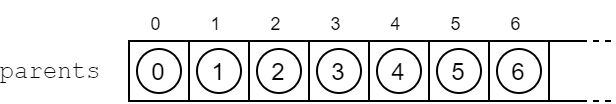
\includegraphics[width=0.7\textwidth]{./images/DisjointSetParentsVector.png}
	\caption{Inizializzazione di \textit{parents} nella classe \textit{DisjointSetBase}}
	\label{fig:disjoint-set-base-parents}
\end{figure}

\noindent Abbiamo realizzato 2 implementazioni diverse di Disjoint Set.
\textit{DisjointSet} adotta la policy \textit{union-by-size} vista a lezione, senza particolari ottimizzazioni. Definisce un membro \textit{std::vector} per salvare le dimensioni dei sottoalberi radicati nei vari nodi salvati, inizializzandolo a 1, come mostrato in figura \ref{fig:disjoint-set-sizes}.

\begin{figure}[htbp]
	\centering
    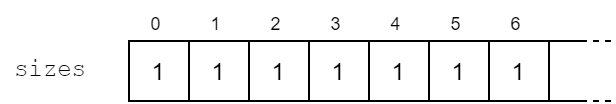
\includegraphics[width=0.7\textwidth]{./images/DisjointSetSizesVector.png}
	\caption{Inizializzazione di \textit{sizes} nella classe \textit{DisjointSet}}
	\label{fig:disjoint-set-sizes}
\end{figure}

\noindent \textit{DisjointSetCompressed}, invece, adotta la policy \textit{union-by-rank} con \textit{path-compression} tramite la tecnica \textit{path-splitting}.
Ad ogni invocazione del metodo \textit{find()} su un nodo $x$, ogni nodo nel percorso da $x$ all'antenato che identifica il set di $x$ è aggiornato per puntare al nodo "nonno". \\
\noindent DisjointSetCompressed definisce un membro \textit{std::vector} per salvare i rank dei dei vari nodi salvati, inizializzando il rank di ogni nodo a 0. Ad ogni invocazione del metodo \textit{unite()} su due nodi $x$ e $y$, ci sono due possibilità:

\begin{enumerate}
    \item Gli alberi di $x$ e $y$ hanno lo stesso rank $\rightarrow{}$ i rank del set che unirà $x$ e $y$ viene incrementato di 1;
    \item Gli alberi di $x$ e $y$ hanno rank diversi $\rightarrow{}$ il set che unirà $x$ e $y$ avrà rank pari a \\ $max\{ rank(find(x)), rank(find(y)) \}$.
\end{enumerate}

La \textit{path-compression} può modificare le altezze degli alberi ad ogni esecuzione, ma non cambierà mai il valore dei rank.
Nonostante sia possibile implementare tecniche di \textit{path-compression} anche con la policy \textit{union-by-size}, abbiamo deciso di cogliere l'opportunità di implementare la policy \textit{union-by-rank}, che non è stata spiegata a lezione. \\

In figura \ref{fig:disjoint-set-union-example} è possibile vedere un esempio di union-by-size implementato dalla classe \textit{DisjointSet}. Analogamente, in figura \ref{fig:disjoint-set-compressed-union-example} è possibile vedere un esempio di union-by-rank con path-splitting implementato dalla classe \textit{DisjointSetCompressed}.

\begin{figure}[h]
	\centering
	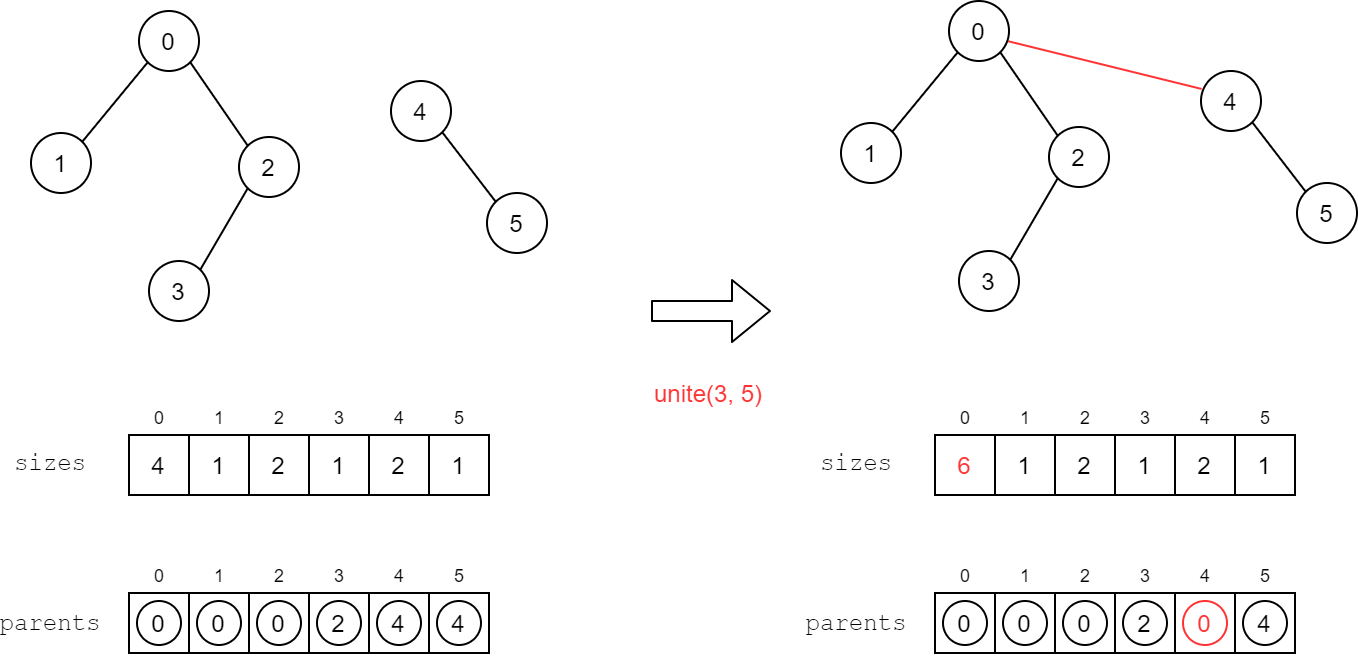
\includegraphics[width=0.7\textwidth]{./images/DisjointSetExample.png}
	\caption{Esempio di unione con DisjointSet}
	\label{fig:disjoint-set-union-example}
\end{figure}

\begin{figure}[h]
	\centering
	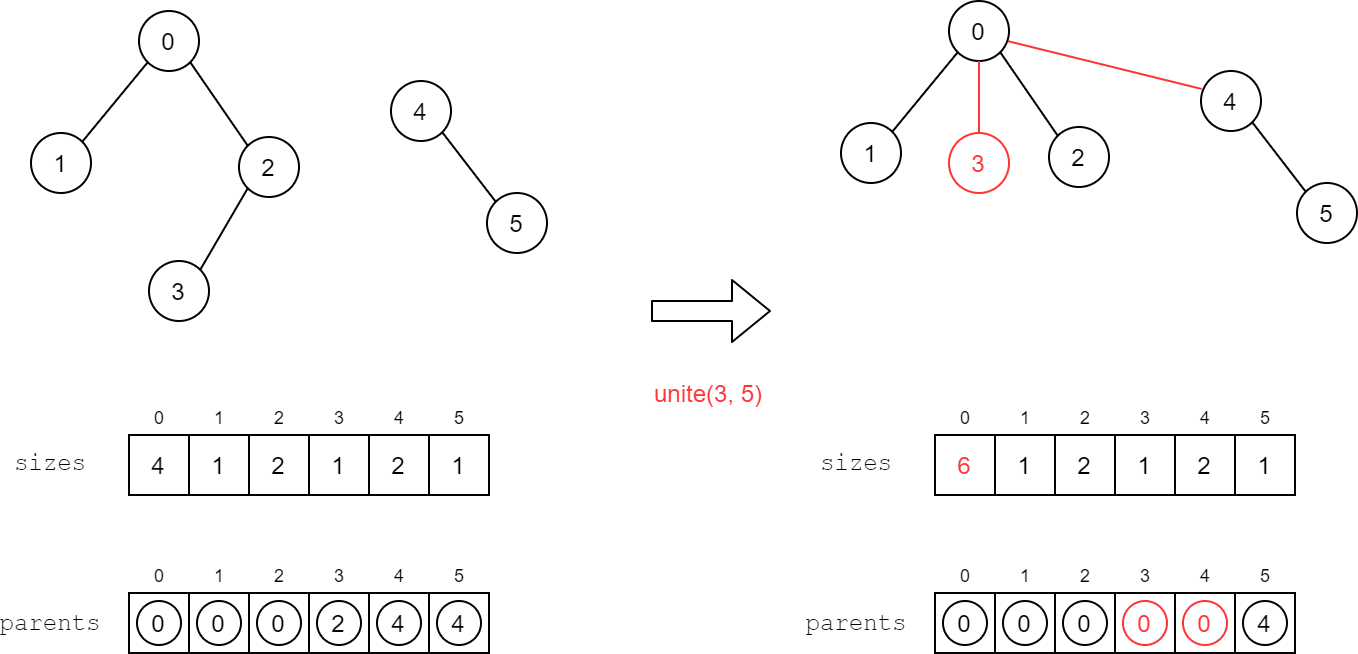
\includegraphics[width=0.7\textwidth]{./images/DisjointSetCompressedExample.png}
	\caption{Esempio di unione con DisjointSetCompressed}
	\label{fig:disjoint-set-compressed-union-example}
\end{figure}